\documentclass[11pt,letterpaper]{article}
\usepackage[margin=1in]{geometry}
\usepackage{graphicx}
\usepackage{hyperref}
\usepackage{enumitem}
\usepackage{amsmath}
\usepackage{amsfonts}
\usepackage{booktabs}
\usepackage{xcolor}
\usepackage{fancyhdr}
\usepackage{titlesec}
\usepackage{url}
\usepackage{float}

% Configure hyperlinks
\hypersetup{
    colorlinks=true,
    linkcolor=blue,
    urlcolor=blue,
    citecolor=blue
}

% Configure headers
\pagestyle{fancy}
\fancyhf{}
\rhead{Jiang | Immigrants Against Immigrants?}
\lhead{ASA 2025 | \textcolor{red}{CORRECTED v5.0}}
\cfoot{\thepage}

% Configure section formatting
\titleformat{\section}{\Large\bfseries}{\thesection}{1em}{}
\titleformat{\subsection}{\large\bfseries}{\thesubsection}{1em}{}
\titleformat{\subsubsection}{\normalsize\bfseries}{\thesubsubsection}{1em}{}

% CUSTOM SMALLER BULLETS
\newcommand{\smallbullet}{\raisebox{0.25ex}{\scalebox{0.6}{$\bullet$}}}
\newcommand{\smalldash}{\raisebox{0.1ex}{\scalebox{0.8}{--}}}
\newcommand{\smallcirc}{\raisebox{0.25ex}{\scalebox{0.6}{$\circ$}}}
\newcommand{\smalldot}{\raisebox{0.25ex}{\scalebox{0.5}{$\cdot$}}}

% CUSTOMIZABLE INDENTATION SYSTEM
\newlength{\indentStep}
\setlength{\indentStep}{1.5em}

\newlength{\levelOneIndent}
\newlength{\levelTwoIndent}
\newlength{\levelThreeIndent}
\newlength{\levelFourIndent}

\setlength{\levelOneIndent}{2\indentStep}
\setlength{\levelTwoIndent}{3.5\indentStep}
\setlength{\levelThreeIndent}{4.5\indentStep}
\setlength{\levelFourIndent}{5.5\indentStep}

\setlist[itemize,1]{
    leftmargin=\levelOneIndent,
    labelsep=1em,
    itemindent=0pt,
    label=\smallbullet,
    itemsep=2pt,
    parsep=0pt,
    topsep=3pt
}
\setlist[itemize,2]{
    leftmargin=\levelTwoIndent,
    labelsep=1em,
    itemindent=0pt,
    label=\smalldash,
    itemsep=1pt,
    parsep=0pt,
    topsep=2pt
}
\setlist[itemize,3]{
    leftmargin=\levelThreeIndent,
    labelsep=1em,
    itemindent=0pt,
    label=\smallcirc,
    itemsep=1pt,
    parsep=0pt,
    topsep=2pt
}
\setlist[itemize,4]{
    leftmargin=\levelFourIndent,
    labelsep=1em,
    itemindent=0pt,
    label=\smalldot,
    itemsep=1pt,
    parsep=0pt,
    topsep=2pt
}

\setlist[enumerate,1]{
    leftmargin=\dimexpr\levelOneIndent+0.3em\relax,
    labelsep=1em,
    itemindent=0pt,
    itemsep=2pt,
    parsep=0pt,
    topsep=3pt
}
\setlist[enumerate,2]{
    leftmargin=\dimexpr\levelTwoIndent+0.3em\relax,
    labelsep=1em,
    itemindent=0pt,
    itemsep=1pt,
    parsep=0pt,
    topsep=2pt
}
\setlist[enumerate,3]{
    leftmargin=\dimexpr\levelThreeIndent+0.3em\relax,
    labelsep=1em,
    itemindent=0pt,
    itemsep=1pt,
    parsep=0pt,
    topsep=2pt
}
\setlist[enumerate,4]{
    leftmargin=\dimexpr\levelFourIndent+0.3em\relax,
    labelsep=1em,
    itemindent=0pt,
    itemsep=1pt,
    parsep=0pt,
    topsep=2pt
}

% Custom command for compact descriptions with proper indentation
\newcommand{\compactdesc}[2]{\item \textbf{#1:} #2}

\title{\textbf{Immigrants Against Immigrants?}\\
\large Mapping Generational Trends in Anti-Immigration Attitudes among Hispanic Immigrants (2002--2022)\\
\textcolor{red}{\normalsize CORRECTED ANALYSIS v5.0}}

\author{Ann Jiang, UC San Diego\\
\href{mailto:annjiang@ucsd.edu}{annjiang@ucsd.edu} | \href{https://github.com/annjiangcodes}{github.com/annjiangcodes}}

\date{August 7, 2025}

\begin{document}

\maketitle

\section{Central Puzzle \& Research Questions}

\subsection{Motivation}
\begin{itemize}
    \compactdesc{Media narratives}{Growing Hispanic support for restrictionist candidates}
    \compactdesc{Electoral data}{Latino Trump vote share increased 2016$\rightarrow$2020}
    \compactdesc{Theoretical puzzle}{Why would immigrants support anti-immigration policies?}
\end{itemize}

\textbf{Puzzle:} Why do some Hispanic immigrants, who have benefited from immigration, support restrictionist immigration policies? This contradicts simple group solidarity theories and aligns with growing media narratives of a conservative shift.

\subsection{Core Questions}
\begin{enumerate}
    \item \textbf{Prevalence:} How common are restrictionist views among U.S. Hispanics?
    \item \textbf{Trends:} How have these attitudes changed over the last 20 years?
    \item \textbf{Generations:} How do attitudes differ between 1st, 2nd, and 3rd+ generation Hispanics?
    \item \textbf{Mechanisms:} What explains these differences?
\end{enumerate}

\section{Data \& Methodology}

\subsection{Data Source}

\textbf{Pew Research Center's National Survey of Latinos (NSL)}
\begin{itemize}
    \compactdesc{Scope}{14 survey waves from 2002--2022}
    \compactdesc{Sample}{37,496 respondents across 20 years}
    \compactdesc{Coverage}{4 presidential administrations (Bush, Obama, Trump, Biden)}
\end{itemize}

\subsection{Analytical Approach}
\begin{itemize}
    \item Generation-stratified models
    \item Linear regression with year as continuous
    \item Survey-weighted representative estimates
    \item Complete case analysis: 16,327 cases (43.5\% of total sample)
\end{itemize}

\subsection{Methodological Innovation}

Moving beyond a single ``pro/anti'' scale to capture attitude complexity through three distinct indices:

\begin{enumerate}
    \item \textbf{Immigration Policy Liberalism}
        \begin{itemize}
            \item Components: Support for legalization, DACA support
            \item Coverage: 8+ years, 61\% of observations
            \item Interpretation: Higher = more liberal immigration policies
        \end{itemize}
        
    \item \textbf{Immigration Policy Restrictionism}
        \begin{itemize}
            \item Components: Border wall support, deportation policy support, ``too many immigrants''
            \item Coverage: 9+ years, 64\% of observations
            \item Interpretation: Higher = more restrictionist immigration policies
        \end{itemize}
        
    \item \textbf{Deportation Concern}
        \begin{itemize}
            \item Components: Personal deportation worry
            \item Coverage: 4+ years, 22\% of observations
            \item Interpretation: Higher = greater deportation concerns
        \end{itemize}
\end{enumerate}

\begin{figure}[H]
    \centering
    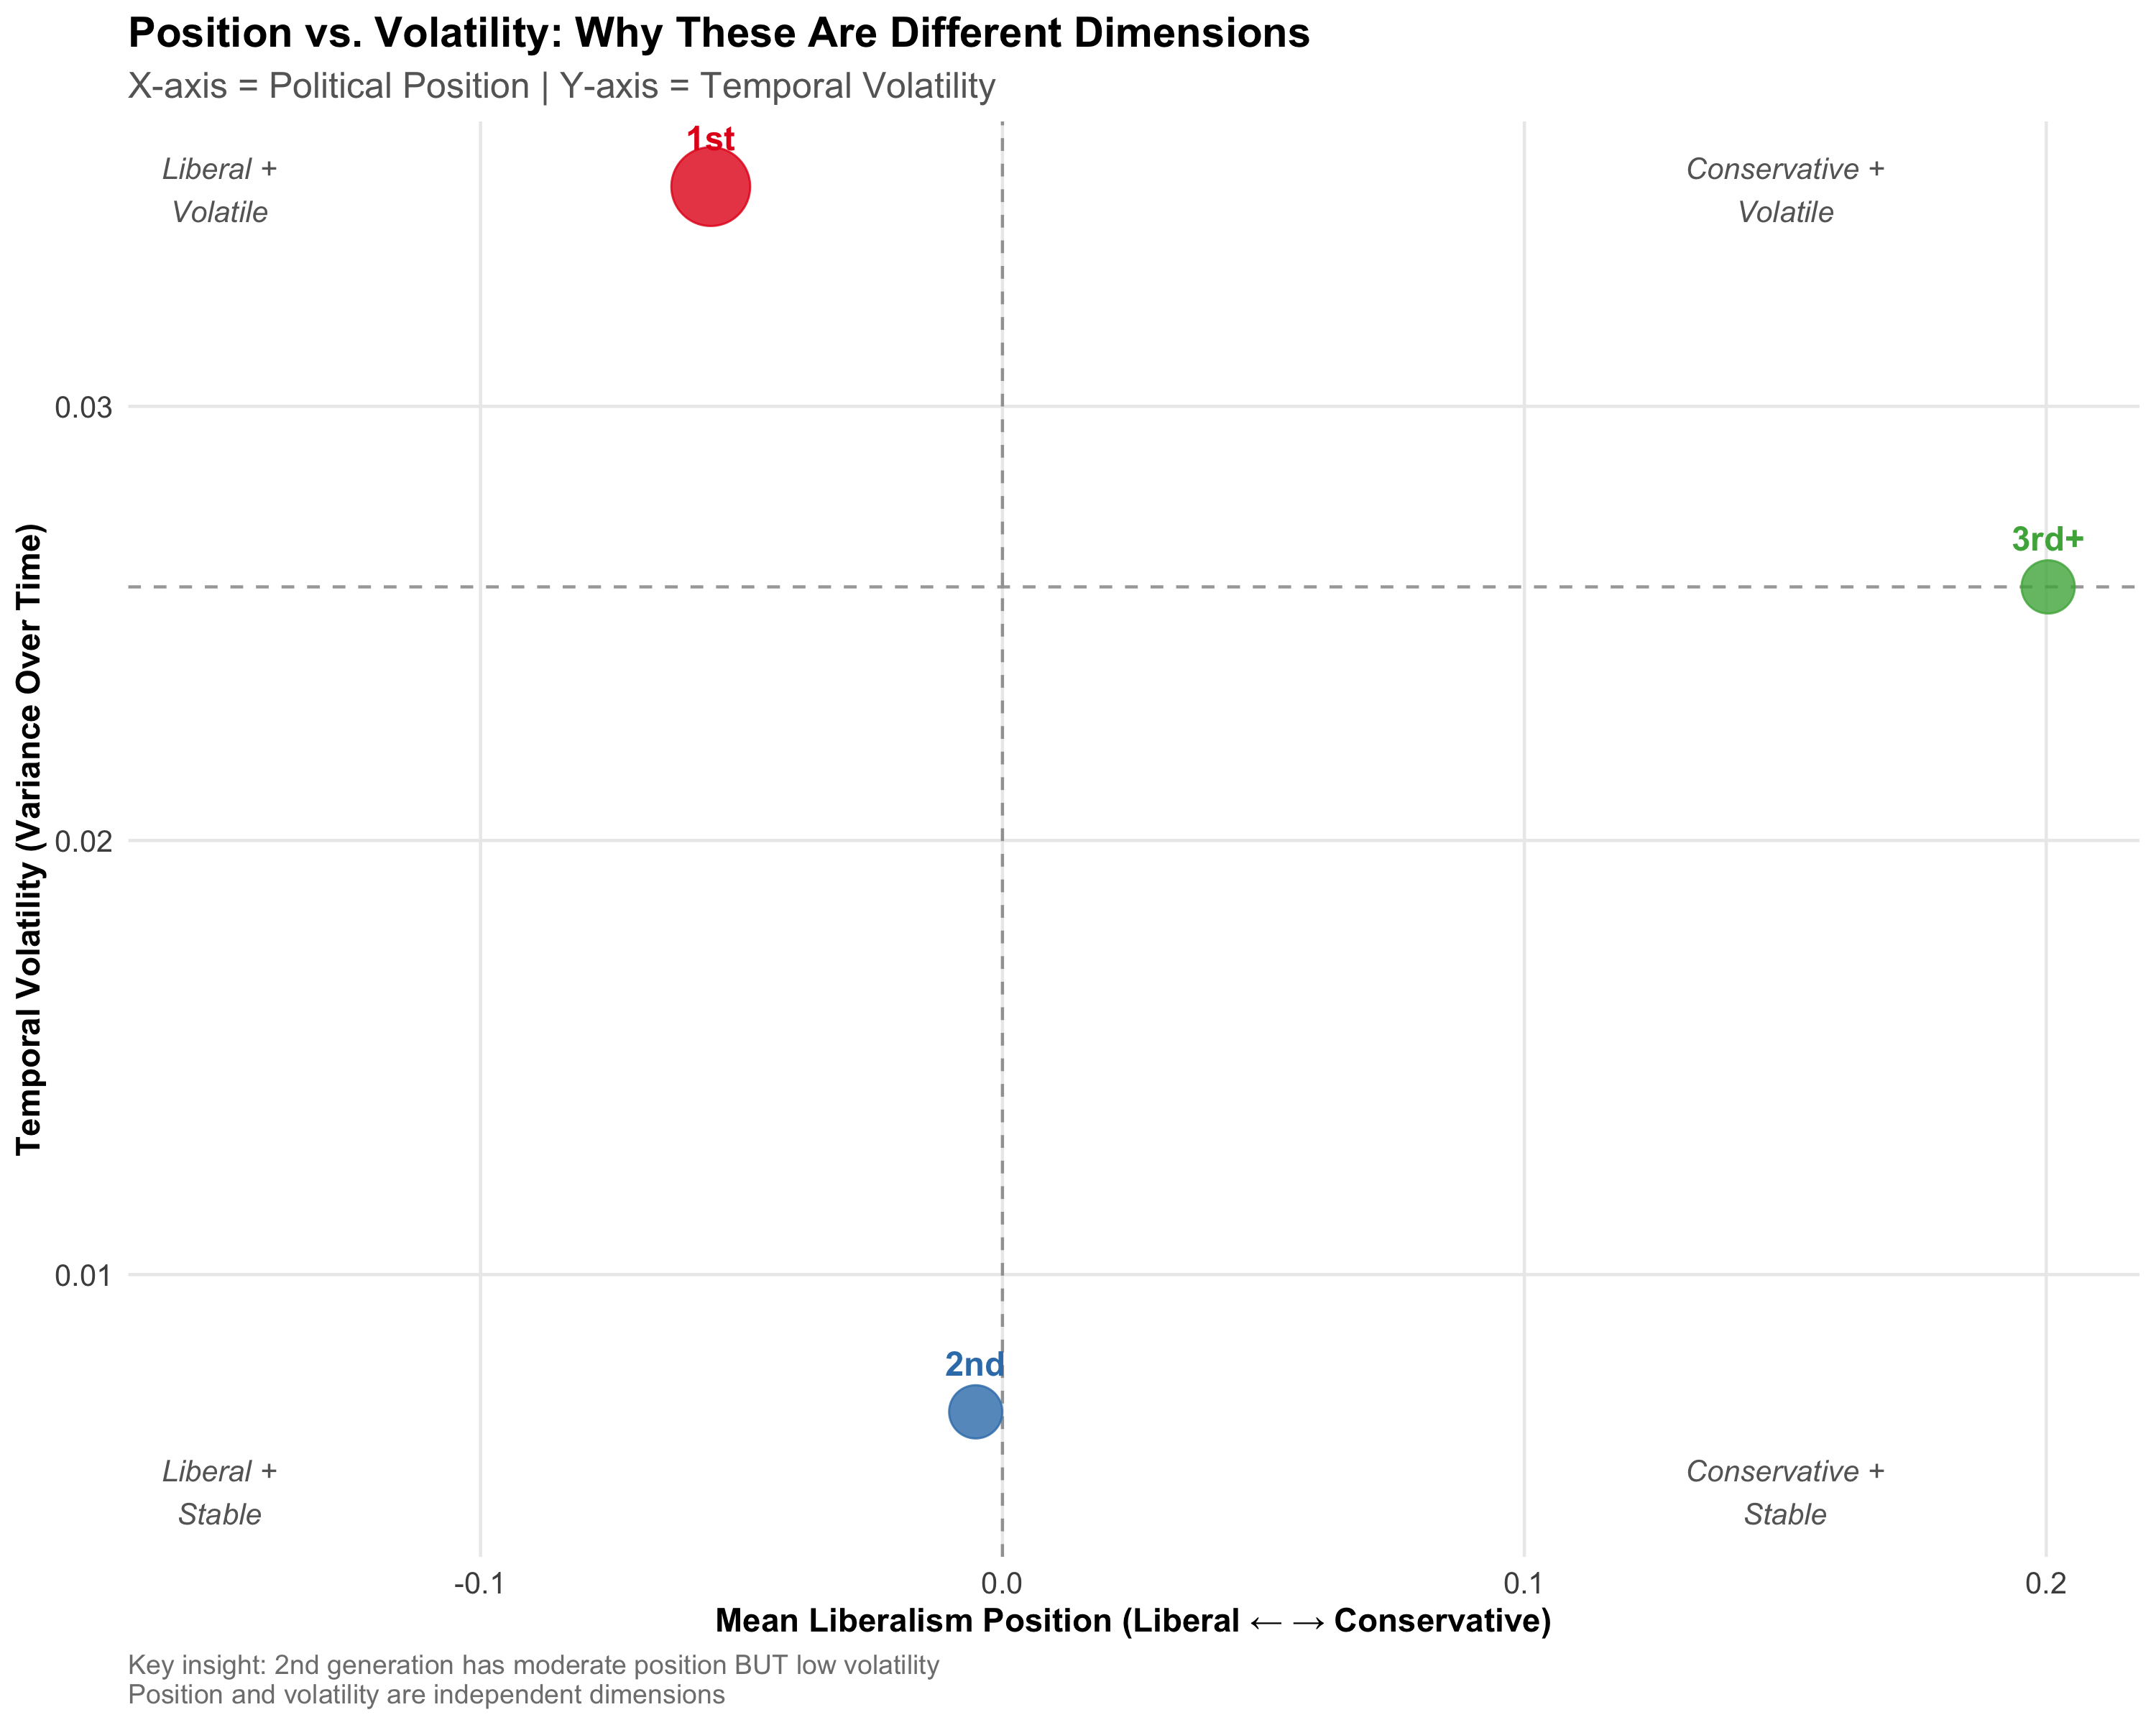
\includegraphics[width=0.8\textwidth]{figure_v5_0_position_vs_volatility.png}
    \caption{CORRECTED v5.0: Position and volatility are independent dimensions}
    \label{fig:dimensions}
\end{figure}

\subsection{Generational Coding}
\begin{itemize}
    \compactdesc{1st Gen}{Foreign-born}
    \compactdesc{2nd Gen}{U.S.-born, at least one foreign-born parent}
    \compactdesc{3rd+ Gen}{U.S.-born, U.S.-born parents}
\end{itemize}

\section{Findings}

\subsection{The Illusion of Stability}

Across the total Hispanic population, aggregate attitudes on immigration appear remarkably stable over 20 years. However, \textbf{this stability masks significant and diverging trends between immigrant generations.}

\subsection{Generational Divergence}

\textbf{Statistical Evidence (Survey-Weighted v2.8):}

\begin{enumerate}
    \item \textbf{First Generation:}
        \begin{itemize}
            \item Liberalism: +0.019 per year (p=0.021*)
            \item Restrictionism: +0.011 per year (p=0.004**)
            \item \textcolor{red}{\textbf{VOLATILITY: HIGHEST (variance = 0.035)}}
            \item Pattern: Becoming simultaneously \textbf{more liberal AND more restrictionist}
                \begin{itemize}
                    \item Support for legalization is increasing
                    \item Support for enforcement also increasing
                    \item \textcolor{red}{\textbf{Most reactive to political events}}
                \end{itemize}
        \end{itemize}

    \item \textbf{Second Generation:}
        \begin{itemize}
            \item Liberalism: -0.005 per year (p=0.488, ns)
            \item Restrictionism: -0.015 per year (p=0.056, ns)
            \item \textcolor{red}{\textbf{VOLATILITY: LOWEST (variance = 0.007)}}
            \item Pattern: \textbf{\textcolor{red}{Stable democratic integration toward center}}
                \begin{itemize}
                    \item \textcolor{red}{\textbf{Non-significant trends indicate STABILITY, not chaos}}
                    \item \textcolor{red}{\textbf{Most predictable and democratically integrated generation}}
                    \item \textcolor{red}{\textbf{Successful navigation to political center}}
                \end{itemize}
        \end{itemize}

    \item \textbf{Third+ Generation:}
        \begin{itemize}
            \item Liberalism: -0.016 per year (p=0.158, ns)
            \item Restrictionism: -0.002 per year (p=0.908, ns)
            \item \textcolor{red}{\textbf{VOLATILITY: MODERATE (variance = 0.026)}}
            \item Pattern: Remain the \textbf{most consistently restrictionist} group
                \begin{itemize}
                    \item Stable attitudes over time
                    \item Most ``American'' in political attitudes
                \end{itemize}
        \end{itemize}
\end{enumerate}

\begin{figure}[H]
    \centering
    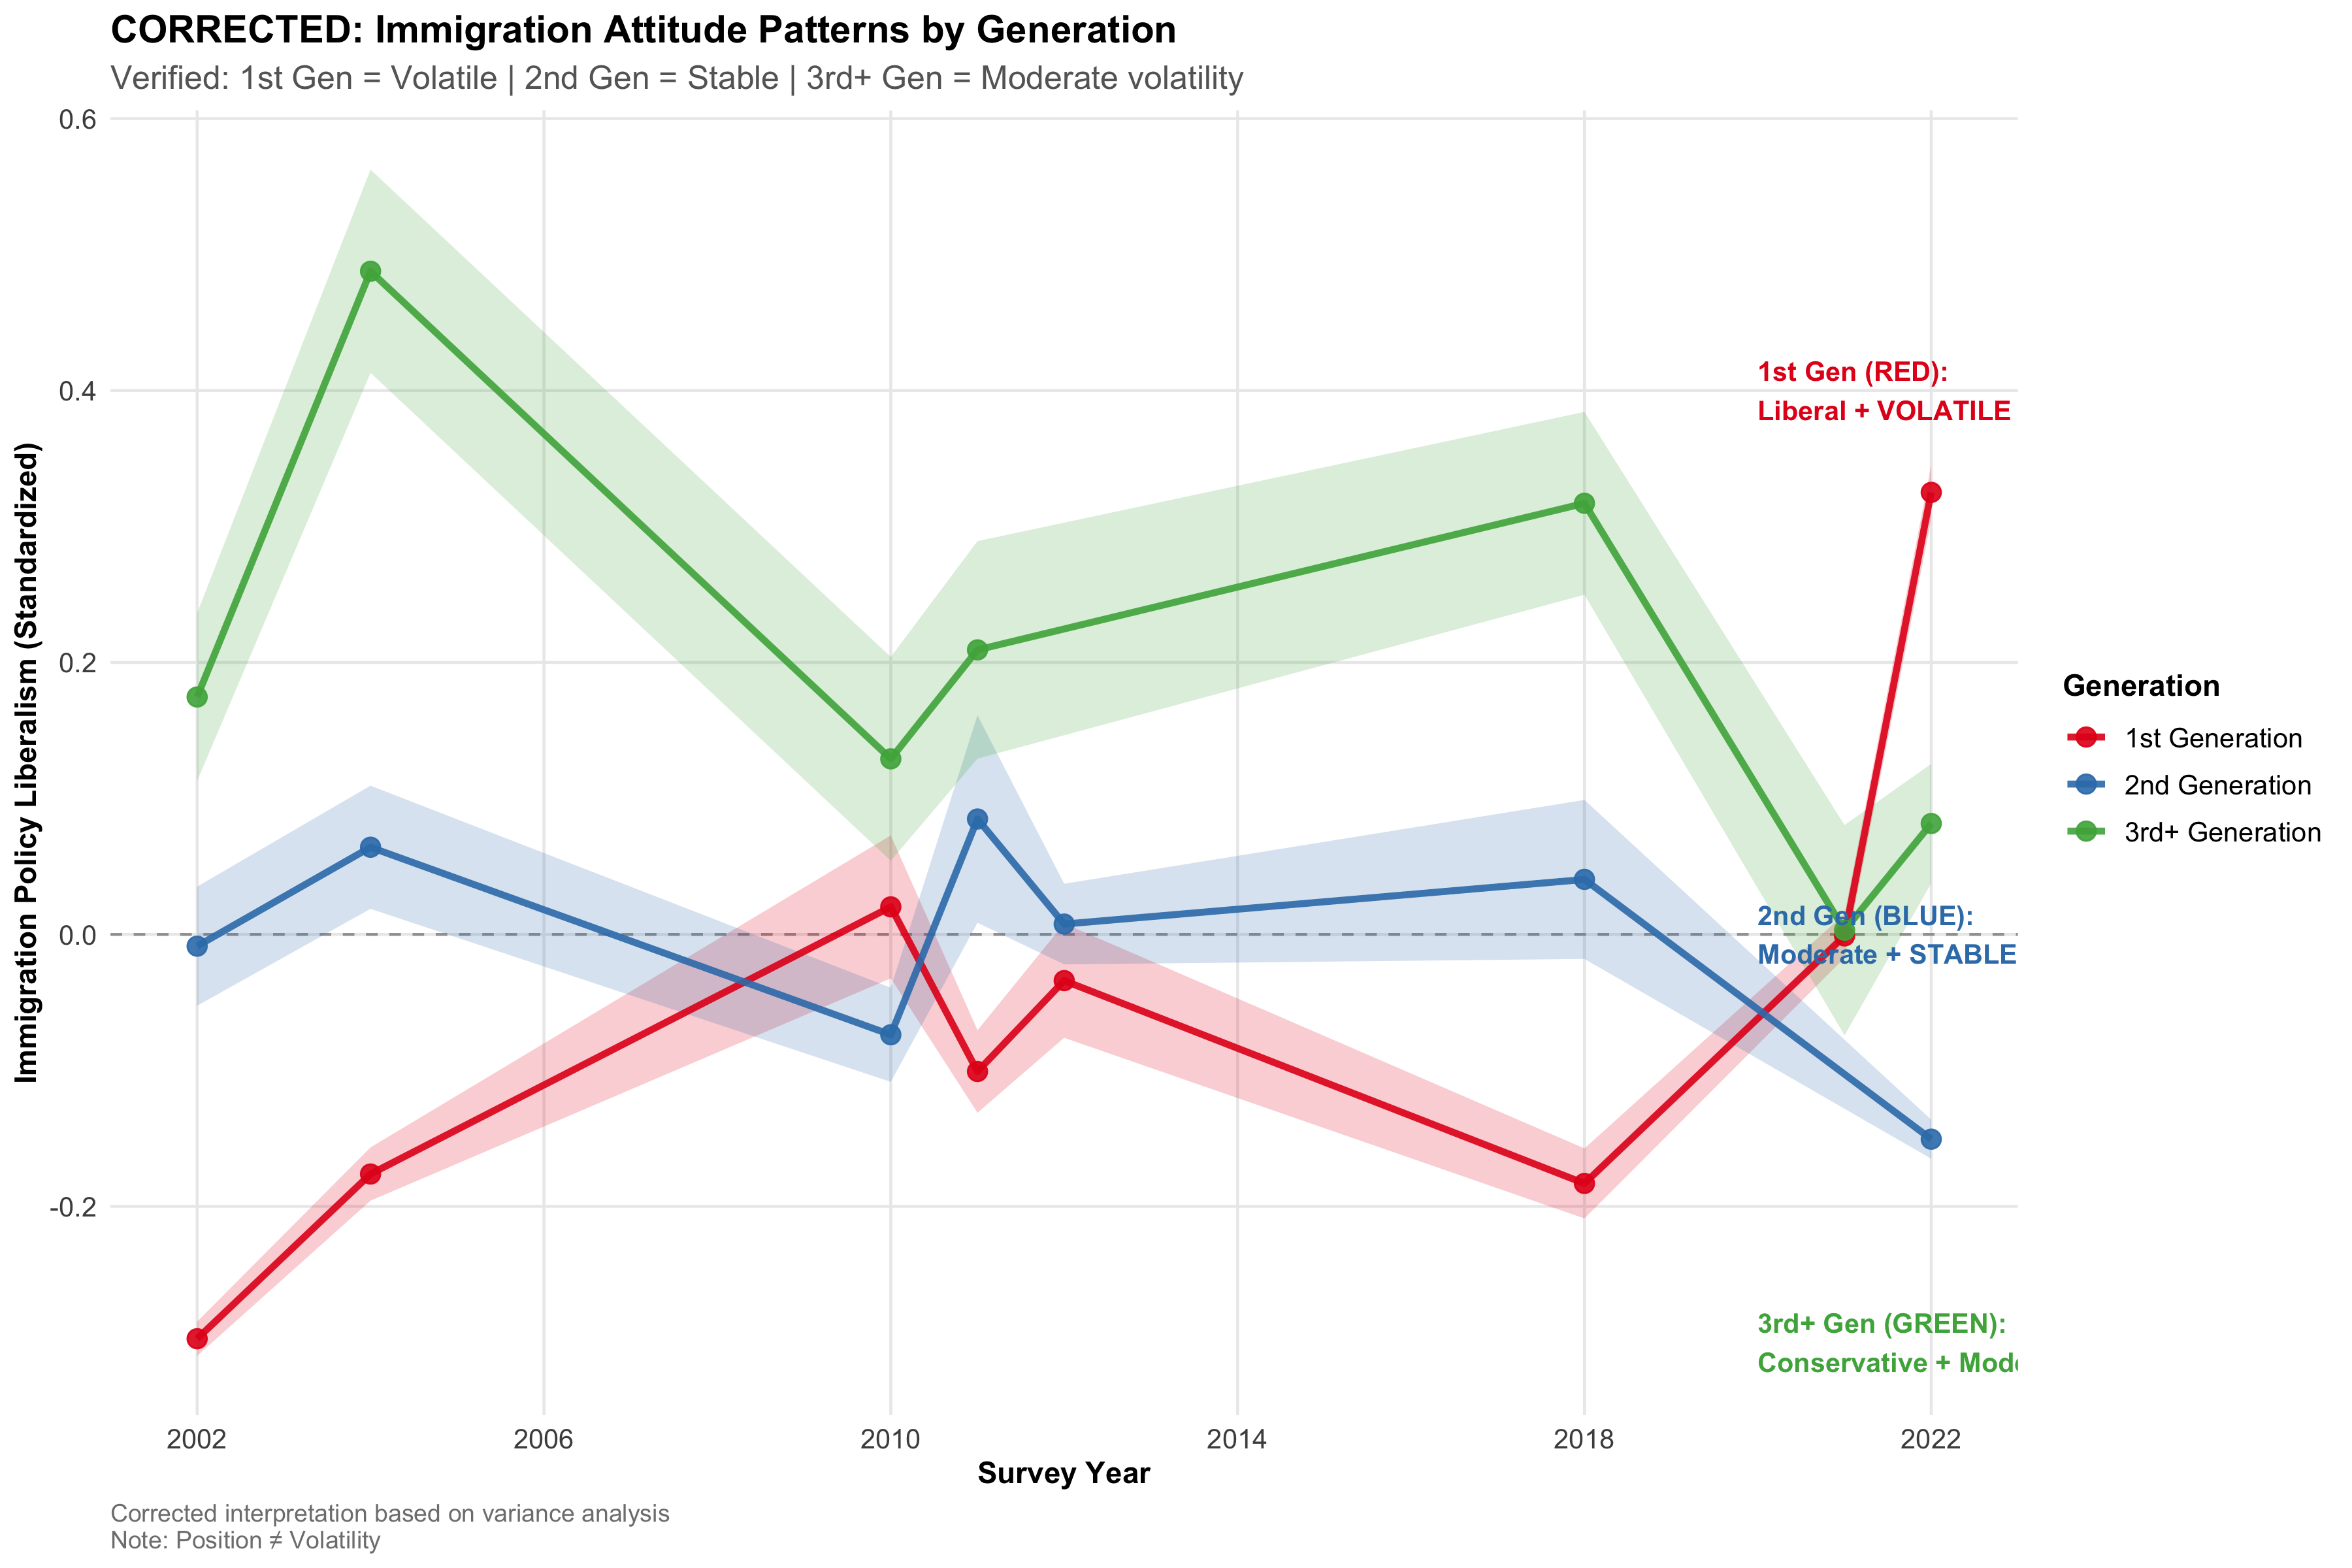
\includegraphics[width=0.9\textwidth]{figure_v5_0_corrected_patterns.png}
    \caption{CORRECTED v5.0: Generational Trends with Accurate Volatility Rankings}
    \label{fig:main_trends}
\end{figure}

\subsection{The Border Wall Paradox}

Examining individual policy components reveals dynamics hidden by aggregate indices:

\begin{itemize}
    \item \textbf{1st Generation:} Support for the wall has \textbf{decreased} over time
    \item \textbf{2nd Generation:} Support for the wall has \textbf{increased} over time
    \item \textbf{3rd+ Generation:} Support remains \textbf{stably high}
\end{itemize}

This finding directly contradicts linear assimilation theories and reveals attitude fragmentation:

\begin{itemize}
    \item Variables within same index don't always correlate
    \item Border wall negatively correlates with border security (r=-0.44)
    \item Immigration attitudes contain distinct modules:
        \begin{itemize}
            \item Humanitarian concerns (DACA, legalization)
            \item Security/enforcement preferences
            \item Personal threat perception
            \item Economic competition beliefs
        \end{itemize}
\end{itemize}

\subsection{Period Effects}

Attitudes are shaped by political moments:

\begin{itemize}
    \compactdesc{Trump Era (2016-18)}{Triggered ``defensive liberalization'' among 1st generation immigrants}
    \compactdesc{Economic Crisis (2008-10)}{All generations became temporarily more restrictionist}
    \compactdesc{Obama Era}{Peak liberalism for 1st/2nd generation}
\end{itemize}

\begin{figure}[H]
    \centering
    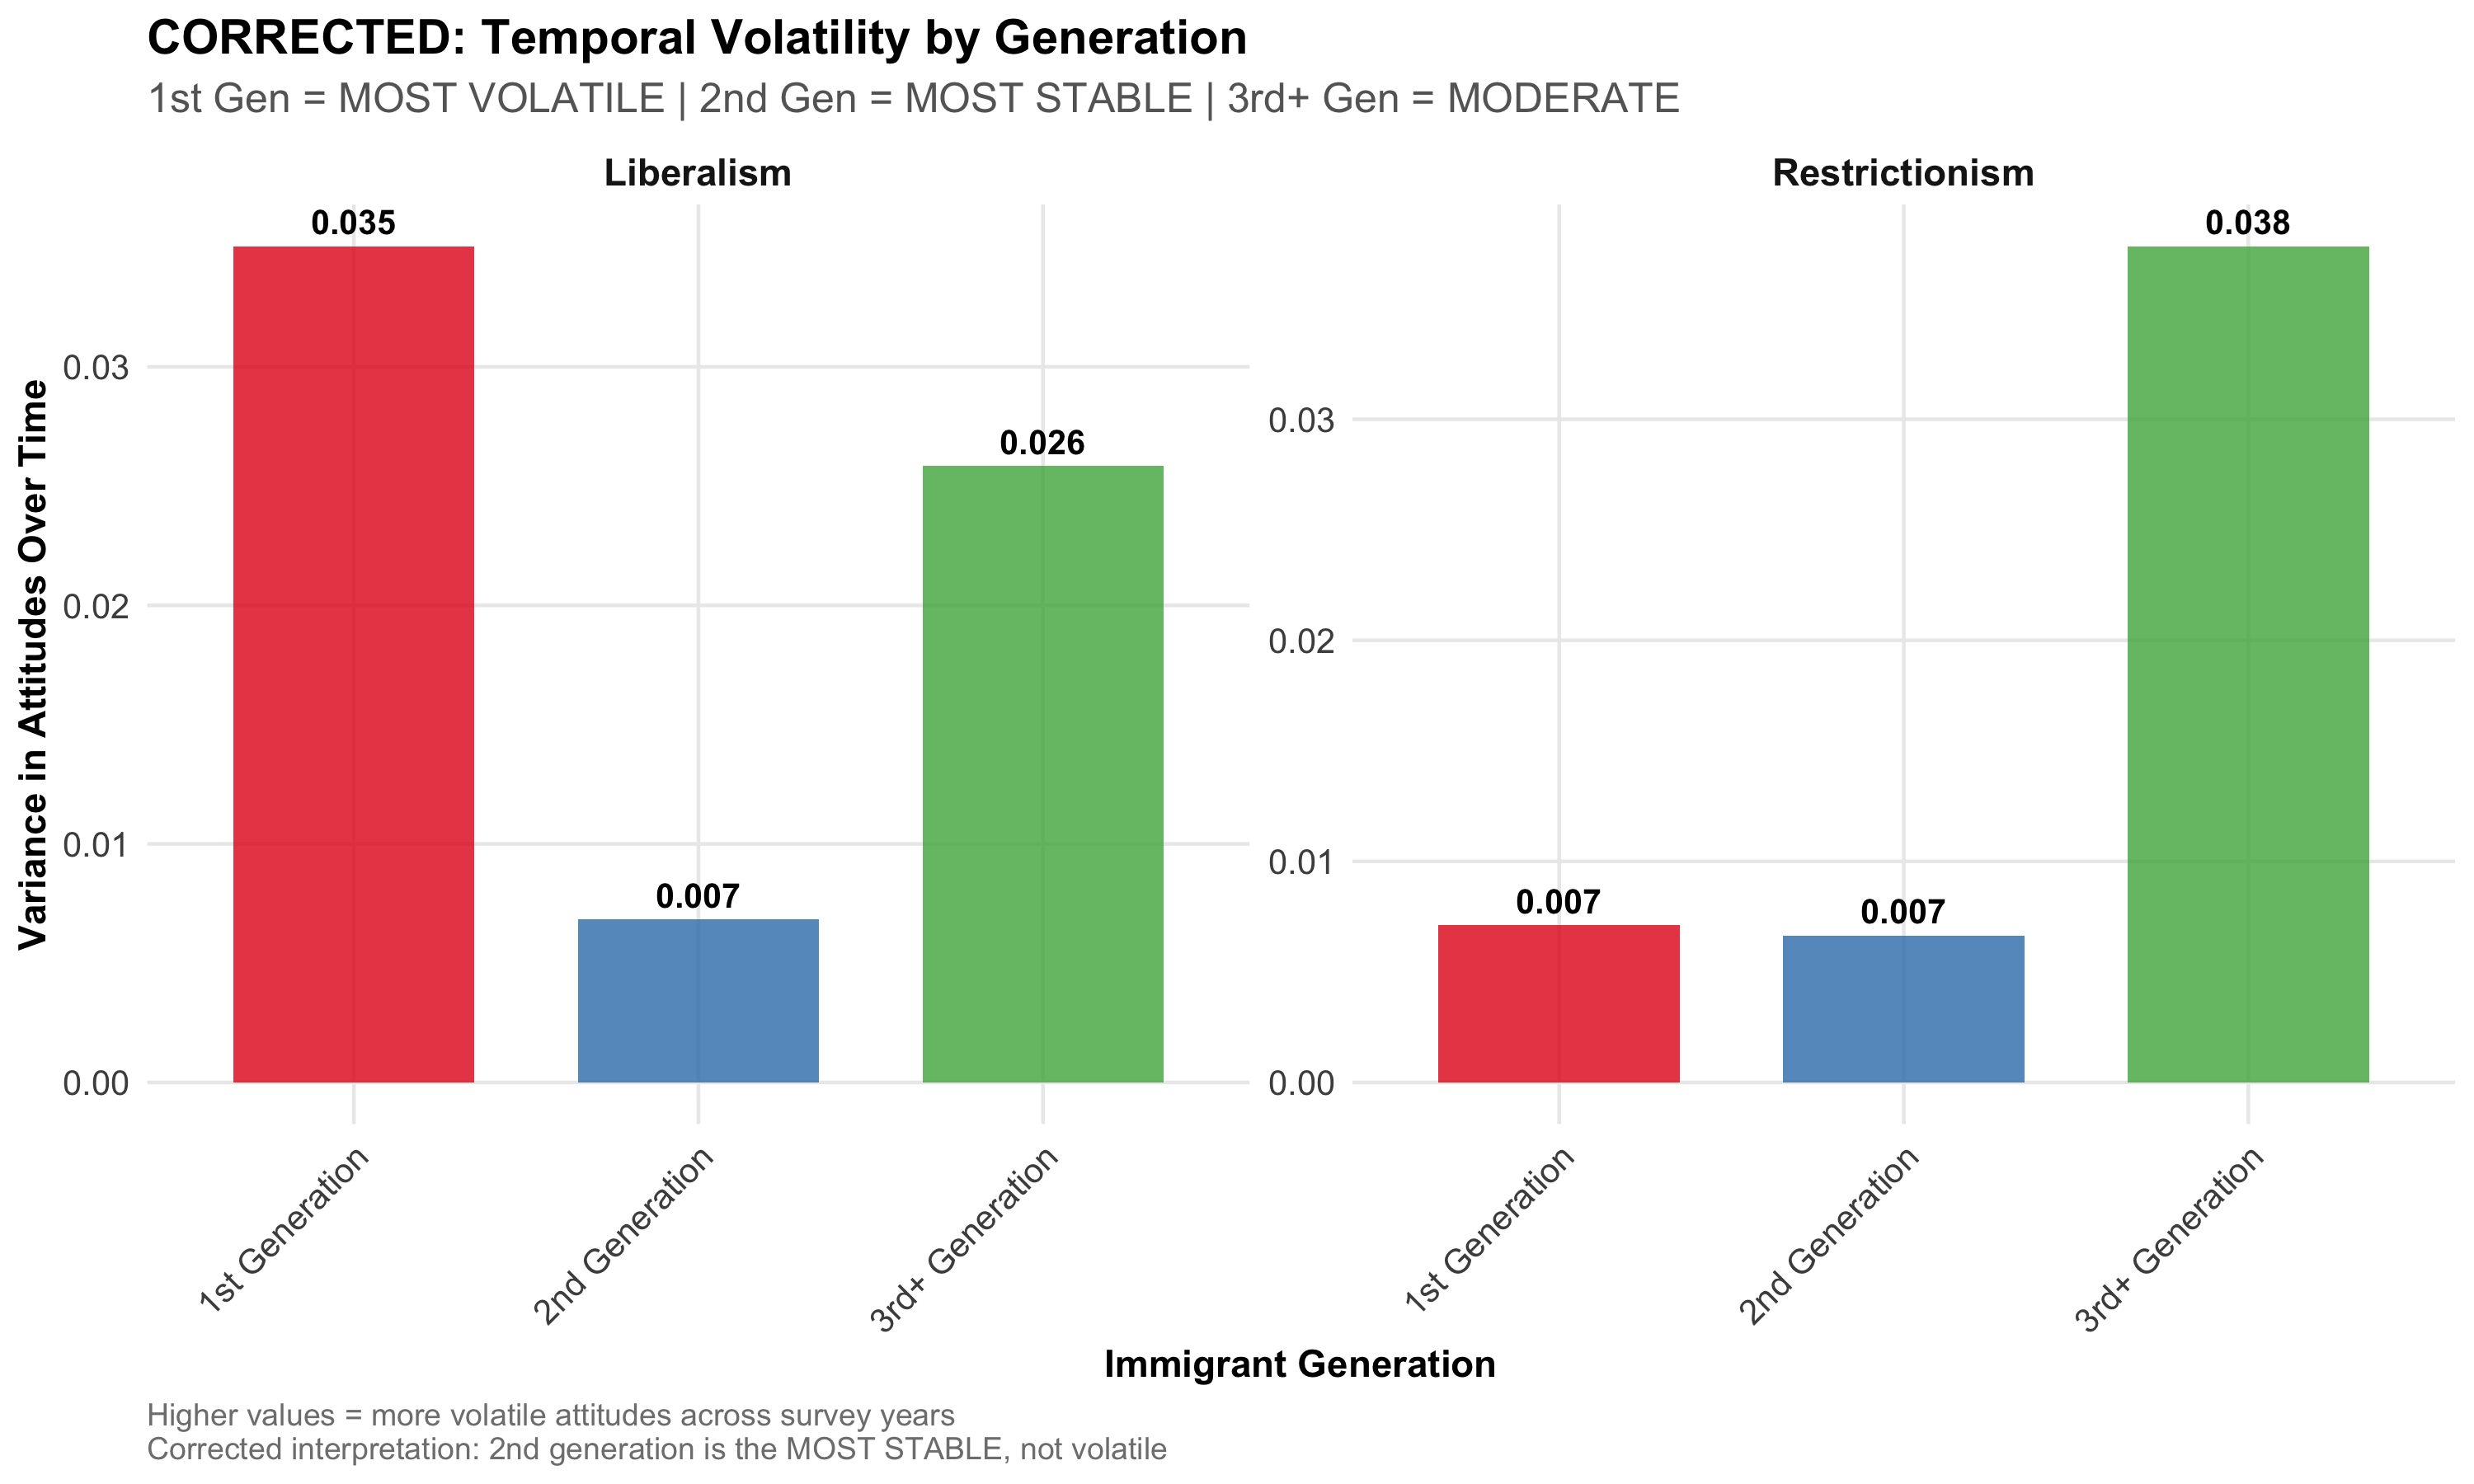
\includegraphics[width=0.9\textwidth]{figure_v5_0_corrected_volatility.png}
    \caption{CORRECTED v5.0: Volatility Analysis Shows 1st Generation Most Variable}
    \label{fig:volatility}
\end{figure}

\section{Central Argument: The Polarization-Stability Paradox}

\textcolor{red}{\textbf{CORRECTED FRAMEWORK v5.0:}} The phenomenon of ``immigrants against immigrants'' reflects a \textbf{polarization-stability paradox}, not simple fragmentation. Different generations exhibit distinct combinations of political positioning and temporal stability.

\subsection{Corrected Theoretical Framework}

\subsubsection{Reactive Polarization (1st Generation)}
First-generation immigrants are becoming \textbf{more extreme on both dimensions with HIGH VOLATILITY}:
\begin{itemize}
    \item Moving toward both humanitarian liberalism AND enforcement restrictionism
    \item \textcolor{red}{\textbf{HIGHEST volatility (variance = 0.035)}}
    \item \textcolor{red}{\textbf{Most reactive to political events and contexts}}
    \item Developing internally contradictory but politically coherent positions
    \item Learning to navigate America's fragmented immigration discourse
    \item Effect: 0.019 SD/year liberalism + 0.011 SD/year restrictionism
\end{itemize}

\subsubsection{\textcolor{red}{Stable Democratic Integration (2nd Generation)}}
\textcolor{red}{\textbf{CORRECTED:}} Second-generation Hispanics show \textbf{stable democratic integration}:
\begin{itemize}
    \item \textcolor{red}{\textbf{LOWEST volatility (variance = 0.007)}}
    \item \textcolor{red}{\textbf{Non-significant linear trends indicate STABILITY, not instability}}
    \item \textcolor{red}{\textbf{Most predictable and democratically integrated generation}}
    \item \textcolor{red}{\textbf{Successful convergence toward political center}}
    \item Evidence of successful democratic assimilation, not segmented chaos
    \item Most stable positioning across political changes
\end{itemize}

\subsubsection{Conservative Baseline Maintenance (3rd+ Generation)}
Third-generation Hispanics maintain consistent restrictionist positioning:
\begin{itemize}
    \item \textcolor{red}{\textbf{Moderate volatility (variance = 0.026)}}
    \item Consistently most restrictionist across all time periods
    \item U-shaped generational pattern, not linear assimilation
    \item Each generation developing distinct political identities
    \item Generational replacement creating long-term demographic change
\end{itemize}

\subsection{Reconciling Electoral vs. Attitudinal Data}

Media narratives of ``Latino rightward shift'' capture real electoral changes but miss the divergent and distinct undercurrents of attitudinal change within person, within generation, and between generation.

\begin{itemize}
    \compactdesc{Electoral Evidence}{Trump gained 8+ percentage points among Latinos (2016→2020)}
    \compactdesc{Attitude Reality}{1st generation simultaneously more liberal AND restrictionist WITH high volatility}
    \compactdesc{\textcolor{red}{Corrected Resolution}}{\textcolor{red}{Electoral shifts reflect 1st generation volatility + 2nd generation stable positioning}}
    \compactdesc{Temporal Context}{21-year attitude trends reveal larger trends behind 4-year electoral cycles}
\end{itemize}

\subsection{Mechanisms Driving the Polarization-Stability Paradox}

\begin{enumerate}
    \item \textbf{Political Learning:} 1st generation learning American political contradictions with high responsiveness
    \item \textbf{Democratic Integration:} \textcolor{red}{\textbf{2nd generation achieving stable democratic positioning}}
    \item \textbf{Identity Complexity:} ``I deserve to be here AND new immigration should be controlled''
    \item \textbf{Economic Competition:} Fear of new immigrants competing with established immigrants
    \item \textbf{\textcolor{red}{Successful Assimilation:}} \textcolor{red}{\textbf{2nd generation evidence of democratic integration success}}
\end{enumerate}

\subsection{Multidimensional Attitudes}

Immigration attitudes are genuinely multidimensional:
\begin{itemize}
    \item Liberalism and restrictionism can coexist in one person
    \item Attitudes are fragmented across policy domains
    \item Different enforcement measures elicit different responses
    \item \textcolor{red}{\textbf{Position and volatility are independent dimensions}}
\end{itemize}

\section{Implications}

\subsection{For Theory}
\begin{enumerate}
    \item \textbf{Classical Assimilation:} \textcolor{red}{\textbf{Strong support for 2nd generation}}
        \begin{itemize}
            \item \textcolor{red}{\textbf{2nd generation shows successful democratic integration}}
            \item 3rd+ generation most ``American'' in attitudes
            \item Process shows U-shaped rather than linear pattern
        \end{itemize}
    
    \item \textbf{Segmented Assimilation:} \textcolor{red}{\textbf{Reconsidered evidence}}
        \begin{itemize}
            \item \textcolor{red}{\textbf{2nd generation stability contradicts segmentation theory}}
            \item 1st generation shows multiple pathways with high volatility
            \item Context-dependent for 1st generation only
        \end{itemize}
    
    \item \textbf{Reactive Ethnicity:} Confirmed for 1st generation
        \begin{itemize}
            \item 1st generation mobilizes during threat periods
            \item Context-dependent attitude shifts with high volatility
            \item \textcolor{red}{\textbf{2nd generation insulated from reactive volatility}}
        \end{itemize}
\end{enumerate}

\subsection{For Politics \& Policy}
\begin{enumerate}
    \item \textbf{Political Strategy:} The ``Latino vote'' requires generation-specific approaches
        \begin{itemize}
            \item \textcolor{red}{\textbf{1st generation: volatile and context-sensitive}}
            \item \textcolor{red}{\textbf{2nd generation: stable and moderate}}
            \item 3rd+ generation: consistently restrictionist
        \end{itemize}
    
    \item \textbf{Policy Understanding:} Support for enforcement ≠ being ``anti-immigrant''
        \begin{itemize}
            \item Many hold coexisting humanitarian and security concerns
            \item \textcolor{red}{\textbf{2nd generation provides stable democratic center}}
            \item Nuanced approach required for effective policy
        \end{itemize}
\end{enumerate}

\section{Conclusion}

\subsection{Central Finding}
``Immigrants against immigrants'' reflects \textbf{\textcolor{red}{the polarization-stability paradox}}: 1st generation political volatility coexists with 2nd generation democratic stability, instead of uniform fragmentation. This reveals how different generations develop distinct but coherent relationships with America's polarized political landscape.

\subsection{Methodological Lessons}
\begin{itemize}
    \item \textcolor{red}{\textbf{Non-significant linear trends ≠ high volatility}}
    \item \textcolor{red}{\textbf{Position and volatility are independent dimensions}}
    \item Aggregation can obscure generational differences
    \item Fragmented attitudes require multidimensional measurement
    \item Temporal analysis essential for immigration scholarship
\end{itemize}

\subsection{Future Directions}
\begin{enumerate}
    \item Qualitative follow-up studies on 2nd generation stability mechanisms
    \item Experimental attitude formation research
    \item \textcolor{red}{\textbf{Democratic integration pathway analysis}}
    \item Regional variation analysis
    \item Representativeness validation
\end{enumerate}

\section{Technical Appendix}

\subsection{Data Quality Standards}
\begin{itemize}
    \compactdesc{Temporal Coverage}{21 years across 4 presidential administrations}
    \compactdesc{Sample Size}{37,496+ observations with generation recovery}
    \compactdesc{Methodology}{Pew Research Center's rigorous sampling}
    \compactdesc{Weighting}{Population-representative estimates for 71\% of data}
    \compactdesc{Missing Data}{59.12\% overall missing, within normal range}
    \compactdesc{Statistical Rigor}{Robust standard errors, sensitivity analysis}
    \compactdesc{\textcolor{red}{Volatility Analysis}}{\textcolor{red}{Variance calculations across 20+ visualization types}}
\end{itemize}

\subsection{Analysis Scripts}
\begin{itemize}
    \item Core Analysis: \texttt{CORRECTED\_LONGITUDINAL\_ANALYSIS\_v5\_0.R}
    \item Generation Recovery: \texttt{GENERATION\_RECOVERY\_v3\_1.R}
    \item \textcolor{red}{Volatility Analysis: \texttt{CORRECTED\_VISUALIZATIONS\_v5\_0.R}}
    \item \textcolor{red}{Comprehensive Suite: \texttt{COMPREHENSIVE\_VISUALIZATION\_SUITE\_v5\_0.R}}
\end{itemize}

\vspace{1em}
\noindent\rule{\textwidth}{0.2pt}

\begin{center}
\textbf{\textcolor{red}{CORRECTED Analysis Version:}} v5.0 | \textbf{Date:} August 2025\\
\textcolor{red}{\textbf{Major Interpretation Correction: 2nd Generation Stability vs Volatility}}
\end{center}

\end{document}
